\subsection{Motor 1}

\subsubsection{Description, type, operation parameters}
%Describe the motor used, provide table with main parameters like resulting voltages->minimum, maximum, nominal, currents, resulting motor power, use figures to show important characteristics.

We are using prototype motors from company TG Drives. They developed prototype motors with special parameters and water cooling. We are using two motors on rear axle (motor 1) and two motors on front axle.
\begin{table}[H]
	\centering
	\caption{General motor 1 data}
	\begin{tabu}{|X|X|}\hline
		Motor Manufacturer and Type: & TG Drives – N5-1600-100-380a-h-special-v2 \\\hline
		Motor principle & PMSM \\\hline
		Maximum continuous power: & 11.5 kW \\\hline
		Peak power: & 35 kW \\\hline
		Input voltage: & 260 V$_AC$ \\\hline
		Nominal current: & 38.2 A \\\hline
		Peak current: & 171 A \\\hline
		Maximum torque: & 48 Nm \\\hline
		Nominal torque: & 11 Nm \\\hline
		Cooling method: & Water \\\hline
	\end{tabu}%
	\label{tab:motors1-general}%
\end{table}%

\begin{figure}[H]
	\centering
	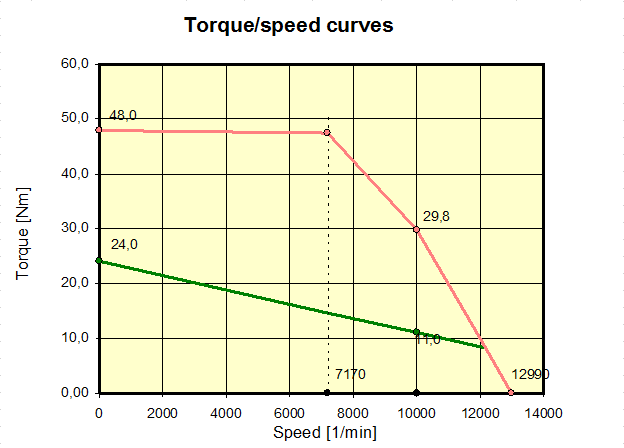
\includegraphics[width=\textwidth]{./img/MOTOR1-torque.png}
	\caption{Rear motor characteristics.}
	\label{fig:torque1}
\end{figure}

\iffalse\begin{itemize}
\item 	Give a plot of power vs. Rpm including a line for nominal and maximum power
\item give a plot of torque vs. rpm including a line for nominal and maximum torque
\end{itemize}\fi

\subsubsection{Wiring, cables, current calculations, connectors}
We use Raychem TR 16-10-0 and TR 16-6-0. There are leadthrough used for cables in motors and connectors Souriau „8STA 0 18 18” are used in Motor controllers.

\subsubsection{Position in car}
%Provide CAD-renderings showing all relevant parts. Mark the parts in the rendering, if necessary and clearly identify the structure used to protect all relevant parts.

Rear motors are situated in the rear-most part of the frame. 

\begin{figure}[H]
	\centering
	\includegraphics[width=\textwidth]{./img/Motor-rear-position.jpg}
	\caption{Rear motor position.}
	\label{fig:Motor-rear-position}
\end{figure}

\subsection{Motor 2}% Front

\begin{table}[H]
	\centering
	\caption{General motor 2 data}
	\begin{tabu}{|X|X|}\hline
		Motor Manufacturer and Type: & TG Drives – M4-0470-90-380a-h-special-water-cooling-lfe-60mm \\\hline
		Motor principle & PMSM \\\hline
		Maximum continuous power: & 4.2 kW \\\hline
		Peak power: & 8.2 kW \\\hline
		Input voltage: & 260 V$_AC$ \\\hline
		Nominal current: & 12.2 A \\\hline
		Peak current: & 67 A \\\hline
		Maximum torque: & 16.2 Nm \\\hline
		Nominal torque: & 4.4 Nm \\\hline
		Cooling method: & Water \\\hline
	\end{tabu}%
	\label{tab:motors2-general}%
\end{table}%

\begin{figure}[H]
	\centering
	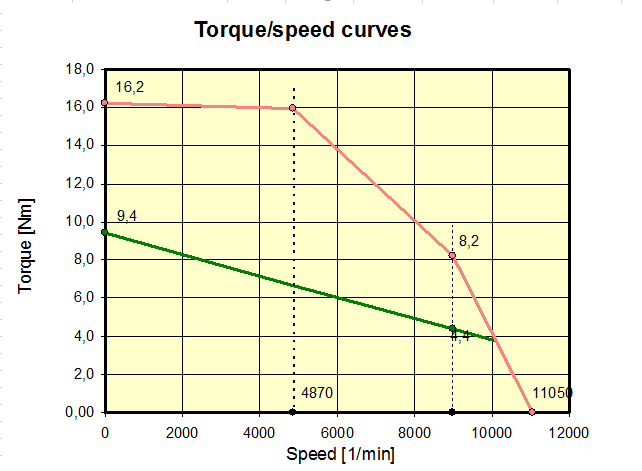
\includegraphics[width=\textwidth]{./img/MOTOR2-torque.png}
	\caption{Front motor characteristics.}
	\label{fig:torque2}
\end{figure}


\subsubsection{Wiring, cables, current calculations, connectors}
We use Raychem TR 16-10-0 and TR 16-6-0. There are leadthrough used for cables in motors and connectors Souriau „8STA 0 18 18” are used in Motor controllers.

\subsubsection{Position in car}
Front motors are situated directly in the front uprights.

\begin{figure}[H]
	\centering
	\includegraphics[width=\textwidth]{./img/Motor-front-position.jpg}
	\caption{Front motor position.}
	\label{fig:Motor-front-position}
\end{figure}


